\documentclass[10pt, a4paper]{article}

\usepackage{lmodern}
\usepackage{tikz}
\usetikzlibrary{arrows.meta, shapes.geometric, positioning, fit, backgrounds, decorations.pathreplacing}
\usepackage[french]{babel}
\usepackage[utf8]{inputenc}
\usepackage[T1]{fontenc}
\usepackage[top=1.8cm, bottom=1.8cm, left=1.8cm, right=1.8cm]{geometry}
\usepackage{amsmath}
\usepackage{booktabs}
\usepackage{hyperref}
\usepackage[protrusion=true,expansion=false]{microtype}
\usepackage[skip=12pt, indent=0pt]{parskip}
\usepackage{array}
\usepackage{caption}
\usepackage{graphicx}
\graphicspath{{figures/}{aasist/exp_result/}}
\usepackage{float}
\usepackage{setspace}
\setstretch{1.0}
\makeatletter
\renewcommand{\section}{\@startsection{section}{1}{\z@}%
  {-8pt \@plus -2pt \@minus -2pt}{4pt \@plus 1pt}%
  {\normalfont\Large\bfseries}}
\renewcommand{\subsection}{\@startsection{subsection}{2}{\z@}%
  {-6pt \@plus -2pt \@minus -1pt}{3pt \@plus 1pt}%
  {\normalfont\large\bfseries}}
\renewcommand{\subsubsection}{\@startsection{subsubsection}{3}{\z@}%
  {-4pt \@plus -1pt \@minus -1pt}{2pt \@plus 1pt}%
  {\normalfont\normalsize\bfseries\itshape}}
\makeatother
\captionsetup{font=small, skip=8pt}
\setlength{\floatsep}{18pt}
\setlength{\textfloatsep}{22pt}
\setlength{\intextsep}{16pt}
\setlength{\abovecaptionskip}{8pt}
\setlength{\belowcaptionskip}{6pt}
% Compacte les listes
\let\oldenumerate\enumerate
\renewcommand{\enumerate}{\oldenumerate\setlength{\itemsep}{0pt}\setlength{\topsep}{2pt}\setlength{\parsep}{0pt}}
\let\olditemize\itemize
\renewcommand{\itemize}{\olditemize\setlength{\itemsep}{0pt}\setlength{\topsep}{2pt}\setlength{\parsep}{0pt}}

\hypersetup{
  colorlinks=true,
  linkcolor=black,
  citecolor=black,
  urlcolor=blue
}

\title{\textbf{Détection de deepfakes vocaux : validation et extension du modèle AASIST}}
\author{Aristide Bailly\\Projet Intégrateur 2A, Télécom Paris, 2025--2026}
\date{}

\begin{document}

\maketitle

\noindent Référence principale : Jung et al., \textit{AASIST: Audio Anti-Spoofing using Integrated Spectro-Temporal Graph Attention Networks}, ICASSP 2022.

\hrule
\vspace{1em}

% ============================================================
\noindent\textbf{Résumé.} La synthèse vocale neuronale permet aujourd'hui de produire des voix artificielles difficiles à distinguer d'une voix réelle, ce qui menace directement les systèmes de vérification du locuteur. Ce projet part du modèle AASIST, un modèle de détection de deepfakes vocaux qui combine une convolution sinusoïdale (SincConv) et deux réseaux d'attention sur graphes (spectral et temporel), pour en valider les performances publiées puis en explorer les limites sur le dataset ASVspoof 2019 LA. J'ai d'abord validé les poids officiels (EER 0,83\,\%, min-tDCF 0,0275, conforme au papier à la quatrième décimale), puis reproduit l'entraînement des quatre architectures de référence (AASIST, AASIST-L, RawGAT-ST, RawNet2), qui retrouvent ou approchent les résultats publiés. L'analyse par type d'attaque montre des profils d'erreur complémentaires entre modèles, en particulier sur les attaques A17/A18 (vocoders neuronaux), ce qui m'a conduit à fusionner les scores de façon pondérée : la fusion atteint 0,73\,\% d'EER, sous le meilleur modèle seul. J'ai ensuite testé trois variantes du protocole d'entraînement (frequency augmentation, noise augmentation, fine-tuning), chacune comparée à AASIST from scratch (1,335\,\%) plutôt qu'aux poids officiels : la frequency augmentation améliore l'EER global d'AASIST ($-$0,19 pt) mais dégrade légèrement celui d'AASIST-L ($+$0,11 pt) tout en améliorant sa robustesse sur A18, et seule la noise augmentation dégrade clairement la performance ($+$0,28 pt). Une expérience de distillation de connaissance (AASIST $\rightarrow$ AASIST-L, $\alpha=0{,}5$, $T=4$) a produit un EER de 1,39\,\%, supérieur de 0,40 pt à l'entraînement from scratch d'AASIST-L (0,99\,\%), ce qui suggère que la distillation n'apporte pas de gain sur ce dataset. La mesure de robustesse au bruit gaussien révèle une dégradation brutale dès 20\,dB SNR (EER 4,20\,\%) et un effondrement quasi-total à 0\,dB (63,10\,\%), cohérent avec l'absence totale de bruit dans ASVspoof 2019 LA.

\smallskip
\noindent\textbf{Mots-clés} : anti-spoofing audio, deepfake vocal, ASVspoof 2019, graph attention network, fusion de systèmes, distillation de connaissance.

% ============================================================
\section{Introduction}

La prolifération des techniques de synthèse vocale neuronale pose un problème de sécurité de plus en plus important, car il est aujourd'hui possible de générer des voix artificielles convaincantes, utilisables pour contourner des systèmes de vérification du locuteur (ASV, \textit{Automatic Speaker Verification}). Ces attaques, appelées \textit{spoofing} ou \textit{deepfakes vocaux}, se divisent en deux grandes catégories : la synthèse vocale (TTS, \textit{Text-To-Speech}) et la conversion vocale (VC, \textit{Voice Conversion}).

Je me suis basé sur le défi ASVspoof, en particulier son édition 2019 qui reste la référence la plus utilisée dans la littérature. Organisé depuis 2015, il standardise l'évaluation des systèmes de contre-mesure (CM, \textit{CounterMeasure}) capables de distinguer une voix authentique (\textit{bona fide}) d'une voix falsifiée (\textit{spoof}).

Publié à l'ICASSP 2022, AASIST (Jung et al.) s'imposait alors comme le meilleur système de détection sur ASVspoof 2019 LA, mais le papier original se concentre sur la performance brute du modèle final et laisse plusieurs questions ouvertes : comment se comporte-t-il en conditions dégradées (bruit) qui n'apparaissent pas dans ASVspoof 2019 LA ? Ses erreurs sont-elles vraiment différentes de celles de modèles plus anciens comme RawNet2, au point qu'une fusion de scores apporte un gain réel ? Et les techniques d'augmentation habituelles sont-elles seulement utiles sur un dataset déjà propre et standardisé comme celui-ci ? Ce sont ces questions, plutôt que la seule performance du modèle, qui structurent ce projet.

Lors de ce projet j'ai :
\begin{itemize}
  \item validé l'implémentation officielle d'AASIST en réévaluant les poids pré-entraînés fournis par les auteurs ;
  \item reproduit l'entraînement des quatre architectures de la même famille de contre-mesures (AASIST, AASIST-L, RawGAT-ST, RawNet2) depuis une initialisation aléatoire ;
  \item analysé les erreurs modèle par modèle et attaque par attaque, pour comprendre où et pourquoi chacun échoue ;
  \item évalué une fusion pondérée des quatre systèmes ;
  \item testé trois variantes du protocole d'entraînement (augmentation fréquentielle, bruit, fine-tuning), chacune isolée pour mesurer sa contribution propre ;
  \item testé une distillation de connaissance (AASIST $\rightarrow$ AASIST-L, résultat : 1,39\,\% EER, supérieur de 0,40 pt au from scratch) ;
  \item mesuré la robustesse au bruit gaussien à cinq niveaux de SNR (0 à 30\,dB), montrant un effondrement à 63\,\% EER à 0\,dB.
\end{itemize}

% ============================================================
\section{Méthode}

\subsection{Architecture AASIST}

AASIST traite un signal audio brut de 4 secondes (64\,600 échantillons à 16\,kHz) et produit un score continu : plus il est élevé, plus le signal est probablement un deepfake. Le pipeline est entièrement différentiable et se décompose en six blocs enchaînés, détaillés ci-dessous avec les dimensions de sortie (\texttt{bs} = taille de batch).

% ---- Figure 1 : pipeline global (vue simplifiée avec dimensions) ----
\begin{figure}[H]
\centering
\scalebox{0.78}{%
\begin{tikzpicture}[
  blk/.style={rectangle, draw=black, fill=#1, rounded corners=4pt,
              text width=2.0cm, align=center, minimum height=1.1cm, font=\small},
  arr/.style={-{Stealth[length=5pt]}, thick},
  lbl/.style={font=\scriptsize, align=center}
]
\node[blk=blue!15]  (inp)  {Audio brut\\{\tiny 64\,600 ech.}};
\node[blk=blue!25,  right=0.7cm of inp]  (sinc) {SincConv\\{\tiny + ResPool}};
\node[blk=blue!35,  right=0.7cm of sinc] (res)  {Encodeur\\résiduel};
\node[blk=orange!30,right=0.7cm of res]  (spl)  {Split S~/~T};
\node[blk=green!30, right=0.7cm of spl]  (gat)  {GAT-S\\GAT-T};
\node[blk=green!50, right=0.7cm of gat]  (htrg) {HtrgGAT\\+ master};
\node[blk=red!25,   right=0.7cm of htrg] (cls)  {Linear\\{\tiny 160$\to$2}};
\foreach \a/\b in {inp/sinc, sinc/res, res/spl, spl/gat, gat/htrg, htrg/cls}
  \draw[arr] (\a) -- (\b);
\node[lbl, below=0.3cm of inp]  {$(64\,600)$};
\node[lbl, below=0.3cm of sinc] {$(1,23,21491)$};
\node[lbl, below=0.3cm of res]  {$(64,23,29)$};
\node[lbl, below=0.3cm of spl]  {$(23,64)$\\$(29,64)$};
\node[lbl, below=0.3cm of gat]  {$(11,64)$\\$(20,64)$};
\node[lbl, below=0.3cm of htrg] {$(5,32)$\\$(10,32)+m$};
\node[lbl, below=0.3cm of cls]  {score};
\node[blk=blue!25,  minimum width=0.5cm, text width=0.5cm, below=1.6cm of inp]  (l1) {};
\node[font=\scriptsize, right=0.2cm of l1] {Extraction de traits};
\node[blk=green!40, minimum width=0.5cm, text width=0.5cm, right=3.5cm of l1]   (l2) {};
\node[font=\scriptsize, right=0.2cm of l2] {Graphes d'attention};
\node[blk=red!25,   minimum width=0.5cm, text width=0.5cm, right=3.5cm of l2]   (l3) {};
\node[font=\scriptsize, right=0.2cm of l3] {Classification};
\end{tikzpicture}}
\caption{Vue schématique du pipeline AASIST avec les dimensions de tenseurs à chaque étape.}
\label{fig:pipeline}
\end{figure}

% ---- Figure 2 : architecture officielle du papier ----
\begin{figure}[H]
\centering
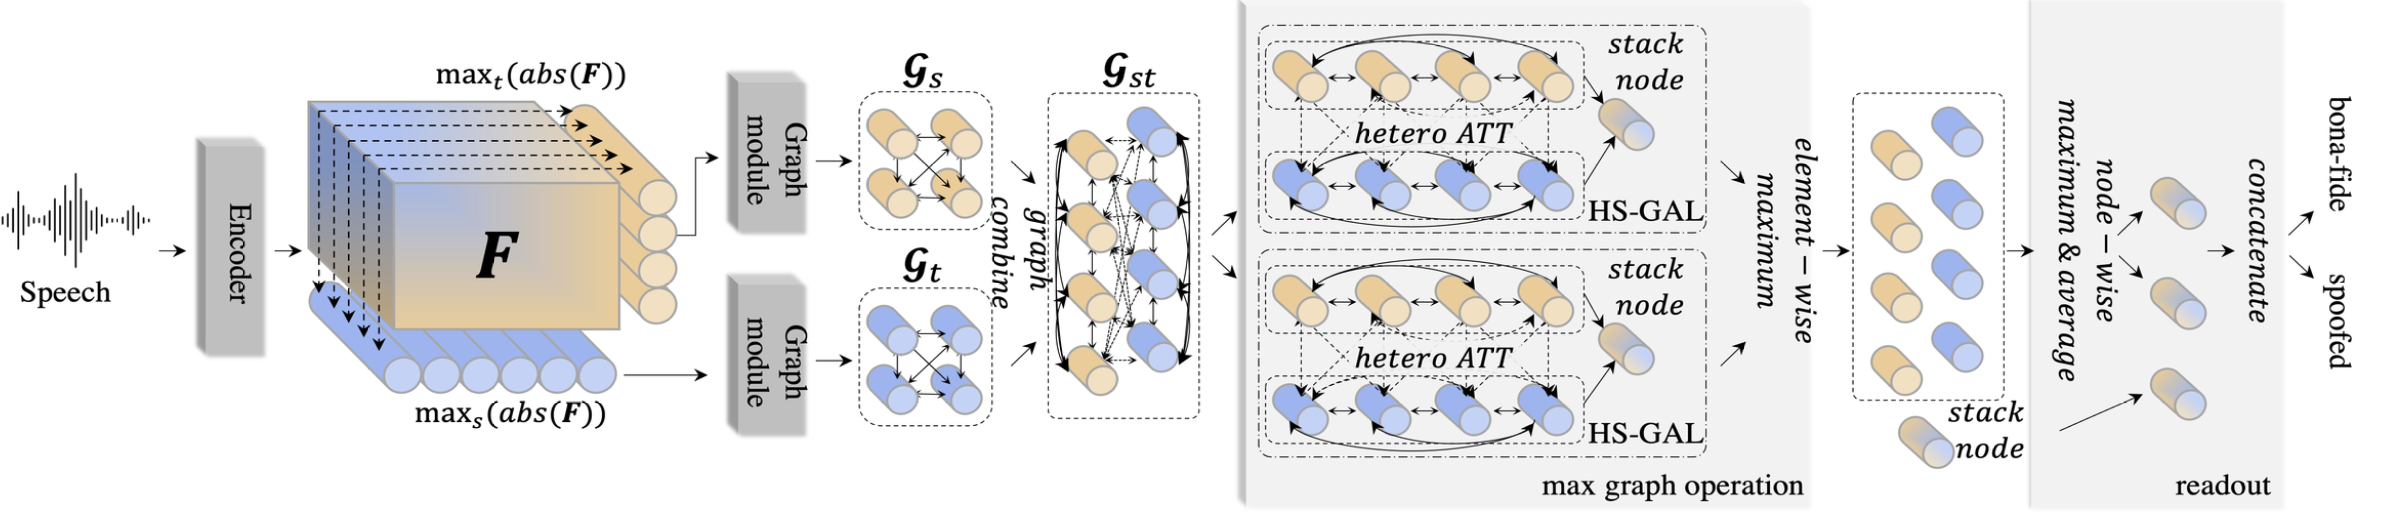
\includegraphics[width=\textwidth]{aasist_architecture.png}
\caption{Architecture AASIST telle que présentée dans le papier original (Jung et al., ICASSP 2022). De gauche à droite : encodeur (SincConv + blocs résiduels), extraction des vues spectrale $\mathcal{G}_s$ et temporelle $\mathcal{G}_t$, fusion hétérogène HtrgGAT avec nœud maître (\textit{stack node}), et agrégation finale (\textit{readout}).}
\label{fig:aasist_paper}
\end{figure}

\subsubsection*{Bloc 1 : SincConv \texttt{(bs, 64600) $\rightarrow$ (bs, 70, 64473)}}

La première couche de convolution ne ressemble pas à une convolution standard. Ses 70 filtres sont contraints à être des passe-bandes sinusoïdaux : chaque filtre est entièrement défini par deux paramètres appris, une fréquence basse $f_{low}$ et une fréquence haute $f_{high}$, au lieu d'apprendre librement l'ensemble de ses coefficients. La forme du filtre est imposée par la physique : c'est un filtre rectangulaire dans le domaine fréquentiel, soit un sinus cardinal dans le domaine temporel, et seules ses bornes sont ajustées par rétropropagation. Cela réduit considérablement le nombre de paramètres par filtre et force une représentation interprétable : en sortie, les 70 canaux correspondent à 70 bandes fréquentielles réparties sur l'échelle mel (0--8\,000\,Hz). Un post-traitement \texttt{abs + MaxPool2D(3×3) + BN + SELU} suit immédiatement : \texttt{abs} élimine le signe pour ne garder que l'intensité, le pooling compresse la représentation d'un facteur $\times 9$, et BN+SELU normalisent et introduisent la non-linéarité. On obtient en sortie \texttt{(bs, 1, 23, 21491)} : un spectrogramme mel grossier, une image fréquence $\times$ temps.

\subsubsection*{Bloc 2 : Encodeur résiduel \texttt{(bs, 1, 23, 21491) $\rightarrow$ (bs, 64, 23, 29)}}

Six blocs résiduels 2D s'enchaînent, chacun composé de deux \texttt{Conv2D(2×3)}, d'une connexion résiduelle (\textit{skip connection}) et d'un \texttt{MaxPool(1×3)} qui divise l'axe temporel par 3. Les canaux augmentent progressivement (1$\rightarrow$32$\rightarrow$64) pour capturer des patterns de plus en plus abstraits, tandis que le temps s'effondre de 21\,491 à 29. La fréquence reste fixe à 23, sans pooling sur cet axe, pour conserver toute l'information spectrale.

\subsubsection*{Bloc 3 : Séparation en deux vues \texttt{(bs, 64, 23, 29) $\rightarrow$ vue S + vue T}}

Le tenseur \texttt{(bs, 64, 23, 29)} encode simultanément l'information fréquentielle (axe 23) et temporelle (axe 29). AASIST les sépare en deux résumés complémentaires par des opérations de max :

\begin{itemize}
  \item \textbf{Vue spectrale} \texttt{(bs, 23, 64)} : max sur l'axe temporel ; pour chaque bande fréquentielle, on retient sa valeur maximale sur toute la durée.
  \item \textbf{Vue temporelle} \texttt{(bs, 29, 64)} : max sur l'axe fréquentiel ; pour chaque instant, on retient la valeur maximale sur toutes les bandes.
\end{itemize}

Ces deux vues sont ensuite traitées par deux graphes d'attention parallèles.

\subsubsection*{Bloc 4 : GAT spectral et temporel \texttt{vue S $\rightarrow$ (bs, 11, 64)} / \texttt{vue T $\rightarrow$ (bs, 20, 64)}}

Un graphe d'attention (GAT, \textit{Graph Attention Network}) permet de modéliser des relations non locales entre éléments d'une séquence. Dans la vue spectrale, chaque nœud du graphe représente une bande fréquentielle (23 nœuds) ; dans la vue temporelle, chaque nœud représente un instant (29 nœuds). Les arêtes entre nœuds ne sont pas fixes : leurs poids sont calculés dynamiquement par un mécanisme d'attention. Pour chaque paire de nœuds $(i, j)$, un coefficient $\alpha_{ij}$ mesure à quel point le nœud $j$ est pertinent pour mettre à jour la représentation du nœud $i$. Le nœud $i$ agrège alors une somme pondérée de ses voisins :
\[
  h_i' = \sum_j \alpha_{ij} \cdot W h_j
\]

L'intérêt par rapport à une convolution est fondamental : une convolution ne voit que des voisins locaux (bandes adjacentes ou instants proches), alors qu'un GAT peut relier n'importe quelle paire de nœuds. Cela permet de capturer des relations longue portée dans le spectre, par exemple une cohérence entre deux bandes fréquentielles distantes qui covarient dans les voix authentiques mais pas dans les deepfakes.

Après le GAT, un \textit{graph pooling} appris élimine les nœuds les moins informatifs en leur attribuant un score de saillance : la vue spectrale passe de 23 à 11 nœuds (ratio 0,5), la vue temporelle de 29 à 20 nœuds (ratio 0,7).

\subsubsection*{Bloc 5 : HtrgGAT, fusion hétérogène \texttt{(bs, 11, 64) + (bs, 20, 64) $\rightarrow$ (bs, 5, 32) + (bs, 10, 32) + nœud maître}}

C'est le composant le plus original d'AASIST et ce qui le distingue principalement de RawGAT-ST, qui traitait les deux branches spectrales et temporelles de façon entièrement indépendante. HtrgGAT construit un graphe \textit{hétérogène} : les nœuds spectraux et temporels sont réunis dans un même graphe, avec des types d'arêtes différents selon la nature de la relation (spectrale-spectrale, temporelle-temporelle, ou spectrale-temporelle). Cela permet à un nœud de bande fréquentielle d'influencer un nœud temporel, et vice versa, ce qui est impossible dans deux graphes homogènes séparés. L'hypothèse sous-jacente est que les deepfakes introduisent des incohérences entre les deux domaines que seule une modélisation croisée peut détecter.

L'élément clé est le \textbf{nœud maître} : deux nœuds apprenables $m_1$ et $m_2$ sont ajoutés au graphe, connectés à tous les autres nœuds. Leur rôle est d'agréger un résumé global de l'ensemble du signal et de le redistribuer comme signal de contexte à chaque nœud lors de chaque couche d'attention. Le mécanisme est appliqué deux fois en parallèle (deux têtes d'attention), et on conserve le maximum des deux chemins pour chaque nœud.

En sortie, on dispose de trois représentations distinctes : les nœuds spectraux raffinés \texttt{(bs, 5, 32)}, les nœuds temporels raffinés \texttt{(bs, 10, 32)}, et le vecteur du nœud maître \texttt{(bs, 1, 32)}.

\subsubsection*{Bloc 6 : Agrégation et classification \texttt{$\rightarrow$ (bs, 160) $\rightarrow$ (bs, 2)}}

Cinq descripteurs globaux sont extraits des trois représentations de sortie de HtrgGAT par des opérations de max et mean sur les nœuds, puis concaténés en un vecteur de 160 dimensions (5 $\times$ 32). Le max capture les anomalies ponctuelles les plus saillantes ; la mean capture les tendances globales. Une couche linéaire \texttt{Linear(160 $\rightarrow$ 2)} produit deux scores : un score bonafide et un score spoof. C'est la différence entre ces deux scores qui sert de décision finale.

% ------------------------------------------------------------
\subsection{Architectures comparées : RawNet2, RawGAT-ST et AASIST-L}

Trois architectures de la même famille sont reproduites et comparées à AASIST.

\textbf{AASIST-L} est une version allégée d'AASIST ($\sim$85\,k paramètres contre $\sim$297\,k), qui conserve la même structure en 6 blocs mais avec une capacité réduite.

\textbf{RawNet2}~\cite{tak2021} est le précurseur direct : il partage la première couche SincConv d'AASIST, mais la remplace ensuite par des blocs résiduels 1D et une agrégation par GRU (\textit{Gated Recurrent Unit}). Il n'y a aucun graphe : le signal est traité comme une séquence temporelle pure. C'est la baseline la plus simple du groupe, avec $\sim$379\,k paramètres.

\textbf{RawGAT-ST}~\cite{jung2021rawgat} est l'étape intermédiaire entre RawNet2 et AASIST : il introduit deux graphes d'attention séparés, l'un sur l'axe spectral et l'autre sur l'axe temporel, mais les traite de façon \textit{indépendante}. AASIST franchit le pas suivant en les fusionnant via HtrgGAT. RawGAT-ST compte $\sim$462\,k paramètres.

% ---- Figure 2 : comparaison 4 architectures ----
\begin{figure}[H]
\centering
\scalebox{0.72}{%
\begin{tikzpicture}[
  shared/.style={rectangle, draw=black, fill=blue!20, rounded corners=5pt,
                 text width=3.0cm, align=center, minimum height=1.2cm, font=\small},
  core/.style={rectangle, draw=black, fill=#1, rounded corners=5pt,
               text width=3.2cm, align=center, minimum height=1.2cm, font=\small},
  cls/.style={rectangle, draw=black, fill=red!20, rounded corners=5pt,
              text width=2.0cm, align=center, minimum height=1.2cm, font=\small},
  arr/.style={-{Stealth[length=6pt]}, thick, line width=1.2pt},
  lbl/.style={font=\normalsize\bfseries, anchor=east}
]

% ---- RawNet2 (y = 0) ----
\node[lbl] at (0.3, 0) {RawNet2};
\node[shared]       (rn-in)  at (3.2, 0)   {SincConv\\+ ResBlocks 1D};
\node[core=yellow!35](rn-mid) at (7.2, 0)   {GRU\\(séquentiel pur)};
\node[cls]          (rn-cls) at (10.8, 0)  {Linear\\379\,k param.};
\draw[arr] (rn-in)  -- (rn-mid);
\draw[arr] (rn-mid) -- (rn-cls);

% ---- RawGAT-ST (y = -2.8) ----
\node[lbl] at (0.3, -2.8) {RawGAT-ST};
\node[shared]        (rg-in)  at (3.2, -2.8) {SincConv\\+ ResBlocks 2D};
\node[core=green!25] (rg-s)   at (7.0, -2.1) {GAT-S\\(spectral)};
\node[core=green!25] (rg-t)   at (7.0, -3.5) {GAT-T\\(temporel)};
\node[core=green!35] (rg-cat) at (10.0,-2.8) {Concat\\(indépendant)};
\node[cls]           (rg-cls) at (13.2,-2.8) {Linear\\462\,k param.};
\draw[arr] (rg-in)  -- (rg-s);
\draw[arr] (rg-in)  -- (rg-t);
\draw[arr] (rg-s)   -- (rg-cat);
\draw[arr] (rg-t)   -- (rg-cat);
\draw[arr] (rg-cat) -- (rg-cls);

% ---- AASIST (y = -5.8) ----
\node[lbl] at (0.3, -5.8) {AASIST};
\node[shared]        (aa-in)  at (3.2, -5.8) {SincConv\\+ ResBlocks 2D};
\node[core=green!55] (aa-mid) at (7.2, -5.8) {HtrgGAT\\S$\times$T + nœuds maîtres};
\node[cls]           (aa-cls) at (10.8,-5.8) {Linear\\297\,k param.};
\draw[arr] (aa-in)  -- (aa-mid);
\draw[arr] (aa-mid) -- (aa-cls);

% ---- AASIST-L (y = -8.2) ----
\node[lbl] at (0.3, -8.2) {AASIST-L};
\node[shared]        (al-in)  at (3.2, -8.2) {SincConv\\+ ResBlocks 2D};
\node[core=green!30] (al-mid) at (7.2, -8.2) {HtrgGAT\\(version allégée)};
\node[cls]           (al-cls) at (10.8,-8.2) {Linear\\85\,k param.};
\draw[arr] (al-in)  -- (al-mid);
\draw[arr] (al-mid) -- (al-cls);

% ---- Annotation : tronc commun ----
\draw[decorate, decoration={brace, mirror, amplitude=6pt}, thick, blue!50]
  (1.55, -8.8) -- (4.85, -8.8)
  node[midway, below=8pt, font=\scriptsize, blue!70, align=center]
  {tronc commun\\(sauf RawNet2 : 1D)};

% ---- Annotation : bloc différenciateur ----
\draw[decorate, decoration={brace, mirror, amplitude=6pt}, thick, green!60!black]
  (5.55, -8.8) -- (8.85, -8.8)
  node[midway, below=8pt, font=\scriptsize, green!50!black, align=center]
  {bloc différenciateur\\(clé architecturale)};

\end{tikzpicture}}
\caption{Comparaison des quatre architectures. Le tronc commun (SincConv + blocs résiduels) est partagé. La différence principale réside dans le module central : RawNet2 utilise un GRU séquentiel sans graphe, RawGAT-ST deux GAT indépendants (S et T ne s'influencent pas), AASIST les fusionne via HtrgGAT avec nœuds maîtres, et AASIST-L reprend la même structure avec des dimensions réduites.}
\label{fig:comparaison}
\end{figure}

% ------------------------------------------------------------
\subsection{Variantes explorées}
\label{sec:variantes}

Afin d'essayer d'améliorer le modèle AASIST, j'ai testé différentes variantes susceptibles de permettre une amélioration.

\textbf{Variante tirée directement du code officiel :}

\begin{itemize}
  \item \textbf{Frequency augmentation} : en lisant le code des auteurs, j'ai constaté que le paramètre \texttt{Freq\_aug} est implémenté dans \texttt{models/AASIST.py} mais désactivé par défaut. Le mécanisme masque aléatoirement une fenêtre de filtres SincConv (entre 0 et 20 filtres consécutifs) à chaque itération d'entraînement, de façon similaire au SpecAugment appliqué sur l'axe fréquentiel.
\end{itemize}

\textbf{Variante motivée par la question de robustesse :}

\begin{itemize}
  \item \textbf{Noise augmentation} : l'évaluation sous bruit gaussien (section~\ref{sec:robustesse}) mesure la robustesse d'un modèle entraîné sans bruit. Une question complémentaire est de savoir si entraîner avec du bruit modifie ce profil de robustesse. Les deux expériences sont donc conçues ensemble : l'une teste la robustesse à l'inférence, l'autre teste si l'entraînement sous bruit la transfère. Le bruit utilisé est un bruit gaussien additif (bruit blanc), à densité spectrale de puissance constante sur toutes les fréquences.
\end{itemize}

\begin{itemize}
  \item \textbf{Fine-tuning} : cette variante n'était pas prévue initialement. C'est une réaction directe au résultat de noise augmentation (1,618\,\% EER, section~\ref{sec:variantes_res}) : introduire le bruit dès l'initialisation aléatoire perturbe trop l'apprentissage des représentations de bas niveau, et reprendre le meilleur checkpoint officiel pour 30 epochs supplémentaires à $\text{lr}=10^{-5}$ permet d'introduire la robustesse au bruit sans défaire la représentation déjà apprise.
\end{itemize}

Une fusion de scores et une distillation de connaissance sont également testées :

\textbf{Fusion pondérée.} Les scores des quatre modèles sont normalisés (centrés-réduits) puis combinés avec des poids proportionnels à $1/\text{EER}_{eval}$ de chaque modèle, normalisés pour sommer à 1. La motivation est que des modèles d'architectures différentes font des erreurs sur des exemples différents, et leur combinaison devrait donc compenser les faiblesses de chacun.

\textbf{Distillation.} AASIST (teacher, poids officiels gelés) est utilisé pour entraîner AASIST-L (student) avec une perte combinant cross-entropy sur les labels et divergence KL entre les distributions adoucies du student et du teacher :
\[
  \mathcal{L} = \alpha \cdot \text{CE}(\text{student}, y) + (1-\alpha)\cdot \text{KL}(\text{student}_T \,\|\, \text{teacher}_T)
\]
avec température $T=4$ et $\alpha = 0{,}5$. L'idée est qu'AASIST encode dans ses probabilités de sortie une information plus riche que les simples labels binaires, et qu'AASIST-L peut apprendre à imiter ces nuances.

% ============================================================
\section{Protocole expérimental}

\subsection{Dataset}

Le dataset ASVspoof 2019 Logical Access (LA) contient des enregistrements de parole produits par 17 systèmes de synthèse ou de conversion vocale différents, chacun désigné par un code A01 à A19.

Le dataset est divisé en trois partitions :
\begin{itemize}
  \item \textbf{Train} : utilisé pour entraîner le modèle.
  \item \textbf{Dev} : utilisé pendant l'entraînement pour choisir le meilleur checkpoint, sans jamais influencer directement les poids du modèle.
  \item \textbf{Eval} : le test final, jamais vu ni par l'entraînement ni par la sélection de checkpoint ; c'est sur cette partition que tous les résultats du rapport sont calculés.
\end{itemize}

Pour mesurer la capacité du modèle à généraliser à des attaques qu'il n'a jamais vues, les systèmes d'attaque utilisés en train/dev (A01 à A06) sont entièrement différents de ceux utilisés en eval (A07 à A19).

\begin{table}[H]
\centering\small
\caption{Répartition du dataset ASVspoof 2019 LA}
\begin{tabular}{@{}lrr@{}}
\toprule
Partition & Bona fide (voix réelle) & Spoof (voix falsifiée) \\
\midrule
Train & 2\,580 & 22\,800 \\
Dev   & 2\,548 & 22\,296 \\
Eval  & 7\,355 & 63\,882 \\
\bottomrule
\end{tabular}
\end{table}

Le dataset est fortement déséquilibré : environ 90\,\% des fichiers sont spoof, 10\,\% bona fide. Ce déséquilibre est inhérent à la construction du dataset : les enregistrements bona fide proviennent de vrais locuteurs et sont coûteux à collecter, tandis que les données spoof sont générées synthétiquement en grande quantité. Ce déséquilibre est compensé dans l'entraînement par une cross-entropy pondérée (poids 0,9 pour bona fide, 0,1 pour spoof), pour éviter que le modèle apprenne simplement à tout classifier comme spoof.

\subsection{Métriques d'évaluation}

\textbf{EER (\textit{Equal Error Rate})} : le modèle produit un score continu pour chaque audio. Pour prendre une décision, on fixe un seuil : au-dessus, c'est spoof ; en dessous, c'est bona fide. Ce seuil crée toujours deux types d'erreurs : les faux rejets (une vraie voix classée spoof) et les fausses acceptations (un deepfake classé bona fide). L'EER est le taux d'erreur au seuil où ces deux erreurs sont exactement égales. Un EER de 0\,\% signifie une séparation parfaite, 50\,\% correspond à une décision aléatoire.

\textbf{min-tDCF} (\textit{minimum tandem Detection Cost Function}) : c'est la métrique officielle du défi ASVspoof 2019. Elle évalue le CM non pas seul, mais en tandem avec un système ASV, ce qui est plus proche d'un déploiement réel. La formule est :

\[
  \text{t-DCF}(s) = C_1 \cdot P_{miss,CM}(s) + C_2 \cdot P_{fa,CM}(s)
\]

où :
\begin{itemize}
  \item $s$ est le seuil de décision du CM ;
  \item $P_{miss,CM}(s)$ : proportion de deepfakes classés à tort comme bona fide ;
  \item $P_{fa,CM}(s)$ : proportion de voix réelles classées à tort comme spoof ;
  \item $C_1$ et $C_2$ : coefficients de coût qui tiennent compte de $P_{spoof} = 0{,}05$ (les attaques sont rares dans le trafic réel) et des performances du système ASV associé.
\end{itemize}

Le min-tDCF est le minimum de cette fonction sur tous les seuils possibles. Un score sous 0,05 est considéré compétitif. Deux modèles peuvent avoir le même EER mais un min-tDCF différent si leurs erreurs sont réparties différemment entre les deux types, c'est pourquoi le min-tDCF est plus discriminant que l'EER seul.

\subsection{Détails d'implémentation}

Voici les hyperparamètres utilisés pour entraîner tous les modèles. Ils sont fournis par le papier original et les configs officielles d'AASIST.

\begin{table}[H]
\centering\small
\caption{Hyperparamètres d'entraînement}
\begin{tabular}{@{}lll@{}}
\toprule
Hyperparamètre & Valeur & Rôle \\
\midrule
Optimiseur & Adam & Ajuste les poids selon le gradient \\
Learning rate & $10^{-4}$ & Taille du pas à chaque mise à jour \\
$\beta_1, \beta_2$ & 0,9 / 0,999 & Mémoire des gradients passés \\
Weight decay & $10^{-4}$ & Pénalité sur les poids trop grands \\
Scheduler & cosine annealing & Diminue le LR selon une courbe en cosinus \\
SWA & activé en fin d'entraînement & Moyenne les derniers checkpoints \\
Cross-entropy pondérée & 0,1 / 0,9 (bona fide / spoof) & Compense le déséquilibre des classes \\
Batch size & 24 (32 pour RawNet2) & Nombre d'exemples par mise à jour \\
Epochs & 100 & Passages complets sur le jeu d'entraînement \\
Longueur d'entrée & 4\,s (64\,600 ech. à 16\,kHz) & Découpage aléatoire à l'entraînement \\
\bottomrule
\end{tabular}
\end{table}

Les jobs ont été soumis sur le cluster GPU de Télécom Paris.

\subsection{Remarques d'implémentation}

Le code officiel a été publié en 2021 et deux ajustements de compatibilité ont été nécessaires :

\begin{itemize}
  \item \textbf{\texttt{evaluation.py} : \texttt{np.float} supprimé dans NumPy 1.24+.} Le code utilisait \texttt{np.float}, alias de \texttt{float} supprimé depuis NumPy 1.24. Remplacé par \texttt{float}.
  \item \textbf{Configs \texttt{RawGATST\_baseline.conf} et \texttt{RawNet2\_baseline.conf} : chemin de poids inaccessible.} Les deux configs pointaient vers des poids hébergés sur le serveur interne de NAVER, inaccessible depuis l'extérieur. Redirigés vers les checkpoints téléchargés localement.
\end{itemize}

% ============================================================
\section{Résultats et commentaires}

\subsection{Validation des poids officiels}

\begin{table}[H]
\centering\small
\caption{Validation des poids officiels sur ASVspoof 2019 LA eval}
\begin{tabular}{@{}lllll@{}}
\toprule
Modèle & EER (\%) & min-tDCF & EER papier & tDCF papier \\
\midrule
AASIST   & 0,8295 & 0,02753 & 0,83 & 0,0275 \\
AASIST-L & 0,9917 & 0,03090 & 0,99 & 0,0309 \\
\bottomrule
\end{tabular}
\end{table}

Les résultats correspondent au papier à la quatrième décimale près, ce qui valide la mise en place expérimentale (dataset, protocole, code d'évaluation) avant de passer à l'entraînement from scratch.

\subsection{Reproduction de l'entraînement pour les modèles de référence}

\begin{table}[H]
\centering\small
\caption{Entraînements from scratch}
\begin{tabular}{@{}lllll@{}}
\toprule
Modèle & EER (\%) & min-tDCF & Checkpoint & Notes \\
\midrule
AASIST (best eval, ep60)\textsuperscript{‡}  & 1,335 & 0,03871 & 60 (eval)  & référence pour les ablations \\
AASIST (best dev,  ep98)\textsuperscript{‡}  & 1,480 & 0,04951 & 98 (dev)   & protocole standard ; utilisé pour le breakdown \\
AASIST-L   & 0,9917 & 0,0309 & 76 (dev) & Égale le papier à la 4\textsuperscript{e} décimale\textsuperscript{†} \\
RawGAT-ST  & 1,67  & 0,0546  & 85 (dev) & SWA : 1,672\,\% / 0,0551 \\
RawNet2    & 4,231 & 0,113   & 88 (dev) & Pic eval ep54 (4,23\,\%), dégradation ensuite \\
\bottomrule
\end{tabular}

\smallskip
\noindent\textsuperscript{‡}\textit{AASIST présente une divergence dev/eval : l'EER eval atteint son minimum à ep60 (1,335\,\%) puis remonte, tandis que l'EER dev continue de baisser jusqu'à ep98 (best dev). Le checkpoint ep98 est utilisé pour le breakdown (section~4.3) conformément au protocole standard ; ep60 sert de référence pour les ablations (section~4.4) car il représente le meilleur résultat from scratch atteint.}
\end{table}

AASIST et AASIST-L reproduisent les résultats publiés ; RawGAT-ST et RawNet2 approchent les valeurs de la littérature sans qu'une comparaison directe ne soit étayée dans ce rapport. AASIST-L\textsuperscript{†} égale le papier à la quatrième décimale sur les deux métriques : coïncidence réelle, confirmée par la correspondance simultanée de l'EER et du min-tDCF.

\smallskip
\noindent\textsuperscript{†}\textit{Résultat remarquable mais vérifié : l'EER et le min-tDCF sont identiques aux valeurs publiées sur les quatre décimales disponibles. Un seul run a été effectué ; la probabilité d'une telle coïncidence n'est pas nulle étant donné la déterminisme du pipeline d'évaluation une fois le checkpoint fixé.}

AASIST from scratch atteint 1,335\,\% EER (best epoch 98), soit 0,5 point au-dessus des poids officiels (0,83\,\%).

RawNet2 illustre un cas classique de sur-ajustement au dev set : entre l'epoch 54 et l'epoch 88, l'EER dev continue de baisser (0,708\,\% $\rightarrow$ 0,551\,\%) alors que l'EER eval se dégrade (4,23\,\% $\rightarrow$ 5,11\,\% avant de revenir à 4,46\,\%). Le SWA final retombe au niveau de l'epoch 54 (4,231\,\%), ce qui suggère qu'il moyenne efficacement ce sur-ajustement plutôt que de le corriger.

\begin{figure}[H]
\centering

\includegraphics[width=0.72\textwidth]{det_curve_no_ensemble.png}
\caption{Courbe DET des 4 modèles (sans ensemble). La courbe DET trace le taux de fausses acceptations (deepfakes non détectés) en fonction du taux de faux rejets (voix réelles rejetées) pour tous les seuils de décision possibles — plus la courbe est proche du coin bas-gauche, meilleur est le modèle. AASIST domine sur toute la plage de seuils ; RawNet2 reste nettement au-dessus.}
\label{fig:det_no_ens}
\end{figure}

\subsection{Analyse par type d'attaque}

Plutôt que de calculer un EER global sur toutes les attaques à la fois, on isole chaque type d'attaque $A_k$ et on mesure à quel point le modèle arrive à le distinguer des vraies voix. Cela permet de voir sur quelles attaques précisément chaque modèle échoue.

\begin{table}[H]
\centering\small
\caption{EER par attaque pour les 4 modèles, tous entraînés from scratch. Les valeurs AASIST correspondent au checkpoint best dev ep98 (EER global 1,480\,\%, protocole standard).}
\begin{tabular}{@{}lllll@{}}
\toprule
Attaque & AASIST & AASIST-L & RawGAT-ST & RawNet2 \\
\midrule
A09 & 0,08\,\% & \textbf{0,00\,\%} & 0,02\,\% & 0,14\,\% \\
A13 & 0,33\,\% & \textbf{0,20\,\%} & 0,30\,\% & 0,24\,\% \\
A14 & 0,31\,\% & \textbf{0,06\,\%} & 0,59\,\% & 0,63\,\% \\
A11 & 0,75\,\% & \textbf{0,14\,\%} & 0,55\,\% & 1,08\,\% \\
A08 & 0,53\,\% & \textbf{0,20\,\%} & 0,42\,\% & 3,13\,\% \\
A07 & 1,49\,\% & \textbf{0,55\,\%} & 1,53\,\% & 2,76\,\% \\
A16 & 0,80\,\% & \textbf{0,63\,\%} & 1,26\,\% & 0,86\,\% \\
A19 & \textbf{0,68\,\%} & 0,71\,\% & 0,94\,\% & 1,75\,\% \\
A12 & 1,51\,\% & \textbf{0,69\,\%} & 1,67\,\% & 2,77\,\% \\
A10 & 1,73\,\% & \textbf{1,00\,\%} & 1,96\,\% & 2,67\,\% \\
A15 & 1,10\,\% & \textbf{0,57\,\%} & 1,10\,\% & 2,50\,\% \\
A17 & \textbf{1,48\,\%} & 1,92\,\% & 2,18\,\% & 8,08\,\% \\
A18 & 3,37\,\% & \textbf{3,05\,\%} & 4,70\,\% & 14,26\,\% \\
\midrule
\textbf{Moyenne} & 1,09\,\% & \textbf{0,75\,\%} & 1,32\,\% & 3,14\,\% \\
\bottomrule
\end{tabular}
\end{table}

\noindent\textit{Moyenne = moyenne non pondérée des EER par attaque, $\neq$ EER global calculé sur l'ensemble du corpus.}

\medskip
\noindent\textbf{Observations.} A09 et A13 sont triviales pour tous les modèles : ce sont des systèmes TTS plus anciens dont les artefacts sont facilement détectables. À l'autre extrême, A17 et A18 correspondent à des vocoders neuronaux récents et concentrent l'essentiel des erreurs pour tous les modèles.

RawNet2 est de loin le plus en difficulté sur A18 (14,26\,\%) et n'est premier sur aucune attaque.

RawGAT-ST est globalement bon mais souffre également d'A18 (4,70\,\%).

AASIST-L domine sur 11 des 13 attaques et présente le meilleur profil from scratch : son EER moyen par attaque (0,75\,\%) est le plus bas des quatre, avec une bonne homogénéité.

AASIST from scratch reste compétitif sur A09 et A17, mais est plus irrégulier qu'AASIST-L : il est meilleur sur A07 et A17 mais nettement pire sur A11, A12 et A10. Cela illustre que les poids obtenus from scratch n'ont pas convergé aussi bien que les poids officiels, et que l'hétérogénéité des erreurs entre les deux modèles reste exploitable par une fusion.

\subsection{Variantes du protocole d'entraînement}
\label{sec:variantes_res}

Les variantes from scratch sont comparées à AASIST from scratch ep60 (1,335\,\%, meilleur EER eval atteint), et non aux poids officiels (0,83\,\%) : comparer à l'officiel mêlerait l'effet de la modification et le gap naturel entre from scratch et official. Le fine-tuning, qui part des poids officiels, est comparé séparément à ceux-ci.

\begin{table}[H]
\centering\small
\caption{Variantes d'entraînement : chaque modèle comparé à sa propre référence from scratch}
\begin{tabular}{@{}lllll@{}}
\toprule
Variante & EER (\%) & min-tDCF & $\Delta$ EER & Verdict \\
\midrule
\multicolumn{5}{@{}l}{\textit{AASIST — référence : 1,335\,\%}} \\
\midrule
AASIST from scratch (référence)     & 1,335 & 0,03871 & ---                  & --- \\
AASIST + frequency augmentation     & 1,142 & 0,03646 & \textbf{$-$0,19 pt}  & légère amélioration \\
AASIST + noise augmentation         & 1,618 & 0,05401 & +0,28 pt             & dégradation \\
AASIST fine-tuning + noise\_aug\textsuperscript{*} & 1,224 & 0,0383 & +0,39 pt & dégradation \\
\midrule
\multicolumn{5}{@{}l}{\textit{AASIST-L — référence : 0,9917\,\%}} \\
\midrule
AASIST-L from scratch (référence)   & 0,9917 & 0,03090 & ---      & --- \\
AASIST-L + frequency augmentation   & 1,102  & 0,03583 & +0,11 pt & légère dégradation globale \\
\bottomrule
\end{tabular}

\smallskip
\noindent\textsuperscript{*}\textit{Fine-tuning : part des poids officiels (0,83\,\%), $\Delta$ calculé par rapport à ce point de départ.}
\end{table}

\noindent\textbf{Observations.} La frequency augmentation améliore légèrement l'EER global ($-$0,19 pt). La noise augmentation est la seule variante clairement dégradante ($+$0,28 pt) : elle crée un écart entre les conditions d'entraînement (bruité) et d'évaluation (propre), et masque les signatures spectrales fines sur lesquelles AASIST s'appuie. Label smoothing (1,360\,\%, min-tDCF 0,04516) et scheduler adaptatif (1,425\,\%, min-tDCF 0,04647) ont également été testés. En EER, les écarts sont faibles ($+$0,025 pt et $+$0,09 pt) ; en min-tDCF en revanche, la dégradation est notable (respectivement $+$17\,\% et $+$20\,\% par rapport à la référence 0,03871), ce qui nuance le qualificatif de « quasi neutre » sur la métrique de décision.

Le fine-tuning depuis les poids officiels ($+$0,39 pt par rapport à 0,83\,\%) est pire que le point de départ, mais reste meilleur que la noise augmentation from scratch (1,618\,\%) : partir d'une représentation déjà bien apprise limite la dégradation.

Sur l'attaque la plus difficile, A18, la frequency augmentation apporte le gain le plus net :

\begin{table}[H]
\centering\small
\caption{EER sur l'attaque A18 pour chaque variante}
\begin{tabular}{@{}lllll@{}}
\toprule
 & from scratch & freq\_aug & noise\_aug & fine-tuning \\
\midrule
AASIST   & 3,37\,\% & 2,99\,\% & 4,70\,\% & n.d. \\
AASIST-L & 3,05\,\% & \textbf{2,64\,\%} & --- & --- \\
\bottomrule
\end{tabular}
\end{table}

\noindent\textbf{Observations.} Pour AASIST-L, la frequency augmentation dégrade légèrement l'EER global ($+$0,11 pt) mais améliore A18 (3,05\,\% $\rightarrow$ 2,64\,\%). A17 et A18 sont précisément les attaques les plus récentes, correspondant aux vocoders neuronaux de dernière génération. Ce compromis (légère dégradation sur des attaques simples, gain ciblé sur les plus difficiles) pourrait représenter un meilleur équilibre en conditions réelles. Ce résultat reste à confirmer sur plusieurs seeds et sur des datasets plus récents (ASVspoof 5, In-the-Wild).

\medskip
\noindent\textit{Tables complètes par attaque pour chaque variante : annexe~\ref{ann:breakdown}.}

\subsection{Fusion de scores}

Les profils d'erreur complémentaires observés en section~4.3 motivent une fusion des scores des quatre modèles, normalisés (centrés-réduits) puis combinés avec des poids proportionnels à $1/\text{EER}_{eval}$. L'ensemble a été calculé avec les scores des poids officiels AASIST (0,83\,\%), les scores from scratch n'étant pas encore disponibles à ce moment. Les trois autres modèles utilisent leurs scores from scratch.

\begin{table}[H]
\centering\small
\caption{Poids de la fusion pondérée (AASIST : poids officiels ; autres : from scratch)}
\begin{tabular}{@{}lll@{}}
\toprule
Modèle & EER utilisé & Poids \\
\midrule
AASIST    & 0,83\,\% (officiel) & 0,395 \\
AASIST-L  & 0,99\,\% & 0,331 \\
RawGAT-ST & 1,67\,\% & 0,196 \\
RawNet2   & 4,23\,\% & 0,078 \\
\bottomrule
\end{tabular}
\end{table}

\noindent\textbf{Observations.} La fusion pondérée bat tous les modèles individuels, y compris AASIST officiel (0,83\,\%) : 0,73\,\% d'EER et $-$21\,\% de tDCF. Le gain est concentré sur les attaques difficiles (A17 : 1,48\,\% $\rightarrow$ 1,18\,\%, meilleur from scratch individuel étant AASIST ; A18 : 3,05\,\% $\rightarrow$ 2,46\,\%), ce qui confirme que les quatre modèles se trompent sur des exemples au moins partiellement différents. La diversité architecturale (SincConv+GAT vs RawNet2) est plus utile que la performance individuelle de chaque composant.

\begin{figure}[H]
\centering

\includegraphics[width=0.72\textwidth]{det_curve.png}
\caption{Courbe DET avec la fusion pondérée. La fusion (trait épais) passe sous tous les modèles individuels, notamment sur les attaques difficiles.}
\label{fig:det_ens}
\end{figure}

\subsection{Robustesse au bruit}
\label{sec:robustesse}

Le protocole consiste à ajouter du bruit gaussien blanc à l'audio d'évaluation à différents niveaux de SNR (30, 20, 10, 5 et 0\,dB) avec une graine fixée (1234) pour la reproductibilité. Le modèle évalué est AASIST avec ses poids officiels.

\begin{table}[H]
\centering\small
\caption{EER en fonction du niveau de bruit}
\begin{tabular}{@{}ll@{}}
\toprule
SNR (dB) & EER (\%) \\
\midrule
Propre ($\infty$) & 0,83 \\
30 & 1,02 \\
20 & 4,20 \\
10 & 9,36 \\
5  & 25,90 \\
0  & 63,10 \\
\bottomrule
\end{tabular}
\end{table}

\noindent\textbf{Observations.} La dégradation est faible à 30\,dB (+0,2 point), puis s'accélère brutalement entre 20\,dB et 10\,dB ($\times$5 puis $\times$11 par rapport à la référence propre). À 0\,dB, l'EER atteint 63,10\,\%, soit pire qu'un classifieur aléatoire (50\,\% correspondrait à une décision au hasard). Ce résultat s'explique directement par la composition du dataset : ASVspoof 2019 LA ne contient aucun enregistrement bruité, et AASIST s'appuie sur des signatures spectrales fines (bandes SincConv, relations inter-fréquences dans le GAT spectral) qui sont précisément les premières masquées par du bruit additif.

Ce résultat motive rétrospectivement l'expérience de fine-tuning avec noise augmentation : bien que celle-ci dégrade l'EER global (1,22\,\% contre 0,83\,\%), elle pourrait maintenir une meilleure robustesse à des SNR intermédiaires. La comparaison directe n'a pas été réalisée dans ce projet, mais constituerait une suite naturelle.

\subsection{Distillation AASIST $\rightarrow$ AASIST-L}

L'hypothèse testée est qu'AASIST-L distillé depuis AASIST officiel dépasse AASIST-L entraîné from scratch (référence : 0,99\,\% EER). La perte combinée est $\mathcal{L} = 0{,}5 \cdot \text{CE}(\text{student}, y) + 0{,}5 \cdot \text{KL}(\text{student}_T \| \text{teacher}_T)$ avec $T=4$, entraînée sur 100 epochs.

\begin{table}[H]
\centering\small
\caption{Distillation AASIST $\rightarrow$ AASIST-L}
\begin{tabular}{@{}lll@{}}
\toprule
Modèle & EER (\%) & min-tDCF \\
\midrule
AASIST-L from scratch (référence) & 0,9917 & 0,03090 \\
\textbf{AASIST-L distillé} & \textbf{1,390} & \textbf{0,03826} \\
\bottomrule
\end{tabular}
\end{table}

\noindent\textbf{Observations.} La distillation dégrade la performance par rapport à l'entraînement from scratch (+0,40 point d'EER). Sur A18, l'attaque la plus difficile, l'EER distillé (3,56\,\%) reste légèrement au-dessus du from scratch (3,05\,\%) et bien en dessous du label smoothing (6,51\,\%), ce qui suggère que la distillation n'introduit pas les mêmes effets de dilution du signal. Ce résultat s'explique probablement par le fait que le teacher (EER 0,83\,\%) et le student from scratch (EER 0,99\,\%) opèrent déjà dans un régime où les distributions de sortie sont très piquées : il n'y a pas de \textit{dark knowledge} substantiel à transférer, et la distillation se réduit à une contrainte de régularisation supplémentaire sans apport informatif net.

\begin{table}[H]
\centering\small
\caption{Breakdown par attaque : distillation vs from scratch}
\begin{tabular}{@{}lll@{}}
\toprule
Attaque & AASIST-L distillé & AASIST-L from scratch \\
\midrule
A09 & 0,017\,\% & 0,00\,\% \\
A13 & 0,227\,\% & 0,20\,\% \\
A14 & 0,081\,\% & 0,06\,\% \\
A11 & 0,105\,\% & 0,14\,\% \\
A08 & 0,791\,\% & 0,20\,\% \\
A07 & 0,424\,\% & 0,55\,\% \\
A15 & 0,390\,\% & 0,57\,\% \\
A16 & 1,100\,\% & 0,63\,\% \\
A19 & 1,362\,\% & 0,71\,\% \\
A12 & 0,587\,\% & 0,69\,\% \\
A10 & 0,611\,\% & 1,00\,\% \\
A17 & 2,136\,\% & 1,92\,\% \\
A18 & \textbf{3,562\,\%} & \textbf{3,05\,\%} \\
\bottomrule
\end{tabular}
\end{table}

% ============================================================
\section{Limitations}

\textbf{Un seul run par configuration.} Aucune des variantes (section~4.4) n'a été répétée sur plusieurs seeds. Les écarts par rapport à la référence from scratch (freq\_aug $-$0,19 pt, noise\_aug $+$0,28 pt) ne sont pas garantis statistiquement significatifs ; la noise augmentation est cependant assez large pour sembler robuste à la variance d'entraînement.

\textbf{Bruit gaussien blanc uniquement.} Le bruit gaussien est le modèle de dégradation le plus simple ; il ne représente pas des conditions réalistes comme le bruit de foule, la réverbération ou la compression par codec.

\textbf{Pas d'évaluation cross-dataset.} Les quatre modèles sont entraînés et évalués sur ASVspoof 2019 LA exclusivement. Leur généralisation à des datasets plus récents (ASVspoof 5, In-the-Wild) n'est pas mesurée, alors que les attaques A07--A19 sont datées par rapport aux générateurs vocaux de 2024--2025.

\textbf{Pas d'attaque adaptative.} La robustesse face à un adversaire connaissant explicitement l'architecture AASIST (attaques adversariales ciblant les représentations de graphe) n'a pas été étudiée.

% ============================================================
\section{Conclusion}

\textbf{Bilan technique.} Ce projet valide l'implémentation officielle d'AASIST et reproduit l'entraînement des quatre architectures de référence sur ASVspoof 2019 LA. L'analyse attaque par attaque a permis de comprendre quels modèles échouent sur quels types de deepfakes et pourquoi (notamment la vulnérabilité commune sur A17/A18, les vocoders neuronaux), et d'exploiter ces profils complémentaires dans une fusion pondérée qui dépasse tous les modèles individuels (0,73\,\% EER). L'étude des variantes, comparées à la bonne référence (AASIST from scratch), révèle que la plupart des modifications ont un effet faible : seule la noise augmentation dégrade clairement, et la frequency augmentation apporte un léger gain ciblé sur les attaques les plus difficiles.

\textbf{Retour personnel.} Ce projet a été l'occasion de mener mon premier projet d'IA seul. C'est la première fois que j'utilisais un cluster de calcul : soumission de jobs SLURM, gestion des ressources GPU, débogage à distance. C'est aussi la première fois que j'entraînais des modèles de cette taille depuis zéro.

Ce projet m'a permis d'approfondir de manière appliquée des notions vues en cours de deep learning au P3 en les confrontant à des choix concrets. J'ai particulièrement apprécié le travail de comparaison des modèles et d'analyse afin de chercher à comprendre \textit{pourquoi} un modèle est meilleur sur telle attaque et pas une autre.

Ce travail était d'autant plus intéressant qu'il est très différent de ce que je fais en entreprise chez Argon, où mon travail est davantage orienté analyse de données et SQL. Ce projet m'a donné envie de demander à travailler sur des missions plus data science / machine learning.

% ============================================================
\begin{thebibliography}{7}

\bibitem{jung2022}
Jung, J.-w., Heo, H., Tak, H., Shim, H., Chung, J. S., Lee, B.-J., Yu, H.-J., \& Evans, N. (2022).
\textit{AASIST: Audio Anti-Spoofing using Integrated Spectro-Temporal Graph Attention Networks}.
ICASSP 2022.

\bibitem{kinnunen2020}
Kinnunen, T. et al. (2020).
\textit{ASVspoof 2019: A large-scale public database of synthetic, converted and replayed speech}.
Computer Speech \& Language.

\bibitem{jung2021rawgat}
Jung, J.-w. et al. (2021).
\textit{RawGAT-ST: Raw waveform graph attention network for speech anti-spoofing}.
Interspeech 2021.

\bibitem{tak2021}
Tak, H., Patino, J., Todisco, M., Nautsch, A., Evans, N., \& Larcher, A. (2021).
\textit{End-to-end anti-spoofing with RawNet2}.
ICASSP 2021.

\bibitem{kinnunen2018}
Kinnunen, T. et al. (2018).
\textit{t-DCF: A Detection Cost Function for the Tandem Assessment of Spoofing Countermeasures and Automatic Speaker Verification}.
Odyssey 2018.

\bibitem{muller2019}
Müller, R., Kornblith, S., \& Hinton, G. (2019).
\textit{When Does Label Smoothing Help?}
NeurIPS 2019.

\bibitem{wong2020}
Wong, W. (2020).
\textit{What is Label Smoothing?}
Towards Data Science.
\url{https://towardsdatascience.com/what-is-label-smoothing-108debd7ef06}

\end{thebibliography}

% ============================================================
\clearpage
\appendix

\section{Breakdown complet par attaque pour les variantes}
\label{ann:breakdown}

\begin{table}[H]
\centering\footnotesize
\caption{EER par attaque : frequency augmentation et noise augmentation}
\begin{tabular}{@{}llll@{}}
\toprule
Attaque & noise\_aug & AASIST+freq\_aug & AASIST-L+freq\_aug \\
\midrule
A09 & 0,261 & 0,00 & 0,04 \\
A13 & 0,587 & 0,15 & 0,15 \\
A14 & 0,489 & 0,29 & 0,34 \\
A11 & 0,954 & 0,34 & 0,30 \\
A08 & 1,083 & 0,39 & 0,31 \\
A07 & 1,002 & 1,06 & 0,96 \\
A15 & 1,222 & 0,83 & 1,04 \\
A16 & 0,913 & 0,73 & 0,63 \\
A19 & 0,937 & 0,61 & 0,65 \\
A12 & 1,321 & 0,75 & 0,94 \\
A10 & 1,752 & 1,24 & 1,10 \\
A17 & 1,623 & 1,81 & 1,91 \\
A18 & 4,703 & 2,99 & \textbf{2,64} \\
\bottomrule
\end{tabular}
\smallskip

\noindent\textit{Toutes valeurs en \%. Référence AASIST-L no-aug sur A18 : 3,05\,\%.}
\end{table}

\section{Historique d'entraînement RawNet2 (best checkpoints)}

\begin{table}[H]
\centering\small
\caption{Évolution des EER dev et eval pour RawNet2}
\begin{tabular}{@{}llll@{}}
\toprule
Epoch (best dev) & dev EER (\%) & eval EER (\%) & Commentaire \\
\midrule
28  & 0,900 & 5,83 & premier best \\
40  & 0,825 & 5,06 & \\
44  & 0,825 & 4,69 & \\
46  & 0,785 & 4,62 & \\
54  & 0,708 & \textbf{4,23} & meilleur eval \\
70  & 0,708 & 5,11 & dev stable, eval se dégrade \\
73  & 0,628 & 4,53 & \\
82  & 0,551 & 4,65 & \\
88  & 0,551 & 4,46 & best dev, pire eval \\
Final SWA & --- & \textbf{4,231} & $\approx$ niveau ep54 \\
\bottomrule
\end{tabular}
\end{table}

Entre l'epoch 54 et 88, le dev EER continue de baisser tandis que l'eval EER se dégrade : signe net de sur-ajustement au dev set. Le SWA final retombe au niveau de l'epoch 54.

\section{Breakdown EER par attaque}

\begin{figure}[H]
\centering
\begin{tabular}{cc}

\includegraphics[width=0.46\textwidth]{breakdown_AASIST.png} &

\includegraphics[width=0.46\textwidth]{breakdown_AASIST-L.png} \\[2pt]

\includegraphics[width=0.46\textwidth]{breakdown_RawGATST.png} &

\includegraphics[width=0.46\textwidth]{breakdown_RawNet2.png}
\end{tabular}
\caption{EER par attaque pour les 4 modèles (haut gauche : AASIST, haut droite : AASIST-L, bas gauche : RawGAT-ST, bas droite : RawNet2).}
\label{fig:breakdowns}
\end{figure}

\end{document}
